\newpage
\appendix
\section{Posterior distributions}\label{Appendix:PosteriorDistributions}

\begin{figure}[H]
    \centering
    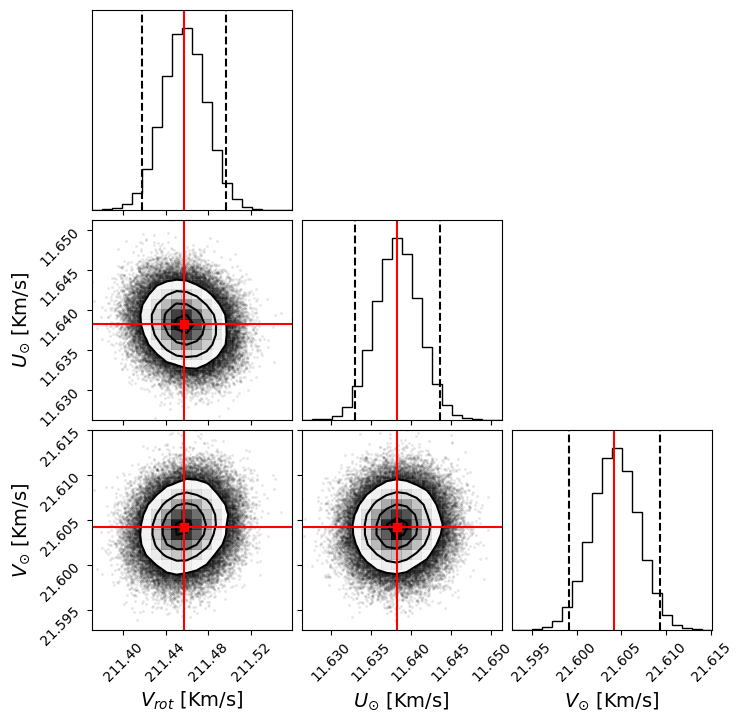
\includegraphics[width = 0.8\linewidth]{Fig/PosteriorSimple.png}
    \caption{Posterior distribution of the parameters for the first model. Red continuous lines indicate the median values found for the respective parameters, while the black dashed ones delimit their 95\% confidence interval.}\label{fig:PosteriorSimple}
\end{figure}

\begin{figure}[H]
    \centering
    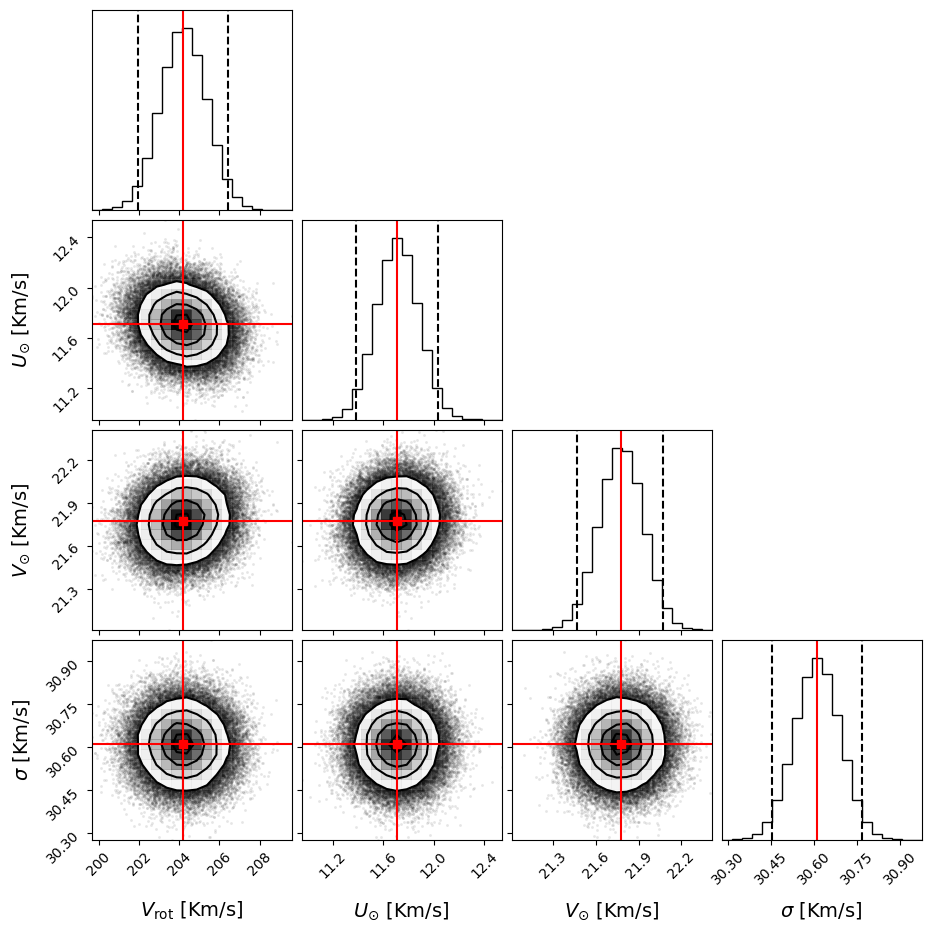
\includegraphics[width = 0.8\linewidth]{Fig/PosteriorFull.png}
    \caption{Posterior distribution of the parameters for the second model. Red continuous lines indicate the median values found for the respective parameters, while the black dashed ones delimit their 95\% confidence interval.}\label{fig:PosteriorFull}
\end{figure}